% !TeX root = ../thuthesis-example.tex

\chapter{绪论}


%
\section{研究背景与意义}

近年来,人工智能技术的发展始终处在快车道,在全球范围内不断取得重大突破,逐渐成为引领性技术。
从统计分析到智能感知再到生成式AI和智能预测,以机器学习为首的人工智能技术持续在不同领域不同任务上发光发热,不断为各行各业带来革命性的转变。
世界各国和主要经济体纷纷加快人工智能战略布局,并相应出台了一系列人工智能发展规划、政策和法律法规。
美国的《国家人工智能研究与发展战略计划》、欧盟的《人工智能法案》、我国的《数字中国建设整体布局规划》和《全球人工智能治理倡议》等一系列战略文件,都明确了人工智能技术的重要性和发展方向,推动着产业界和学术界的技术创新和应用落地。

技术变革的阶段往往也是野蛮生长的阶段,人们关注的焦点大多是如何快速地深化技术,以搏取先发优势和领导者地位。
但当技术面临落地时,工程化、标准化、规模化等方面的诸多挑战开始凸显,制约着其应用推广。
对于机器学习而言,技术增长期常见的“烟囱式”、“手工作坊式”等不成体系的研发模式是造成其应用成本高、管理乱、落地难的重要原因:
一方面,模型研发的工作流程缺乏顶层设计,分工不明确,易出现重复劳动,难以形成有效的团队协作;
另一方面,模型研发过程中产生的资产缺乏统一的存储和管理,资产易流失,经验难传承,难以形成有效的知识沉淀和复用。
本文研究的意义正在于此,通过构建机器学习平台,以工程化的手段来解决这些问题。

\begin{figure}
  \centering
  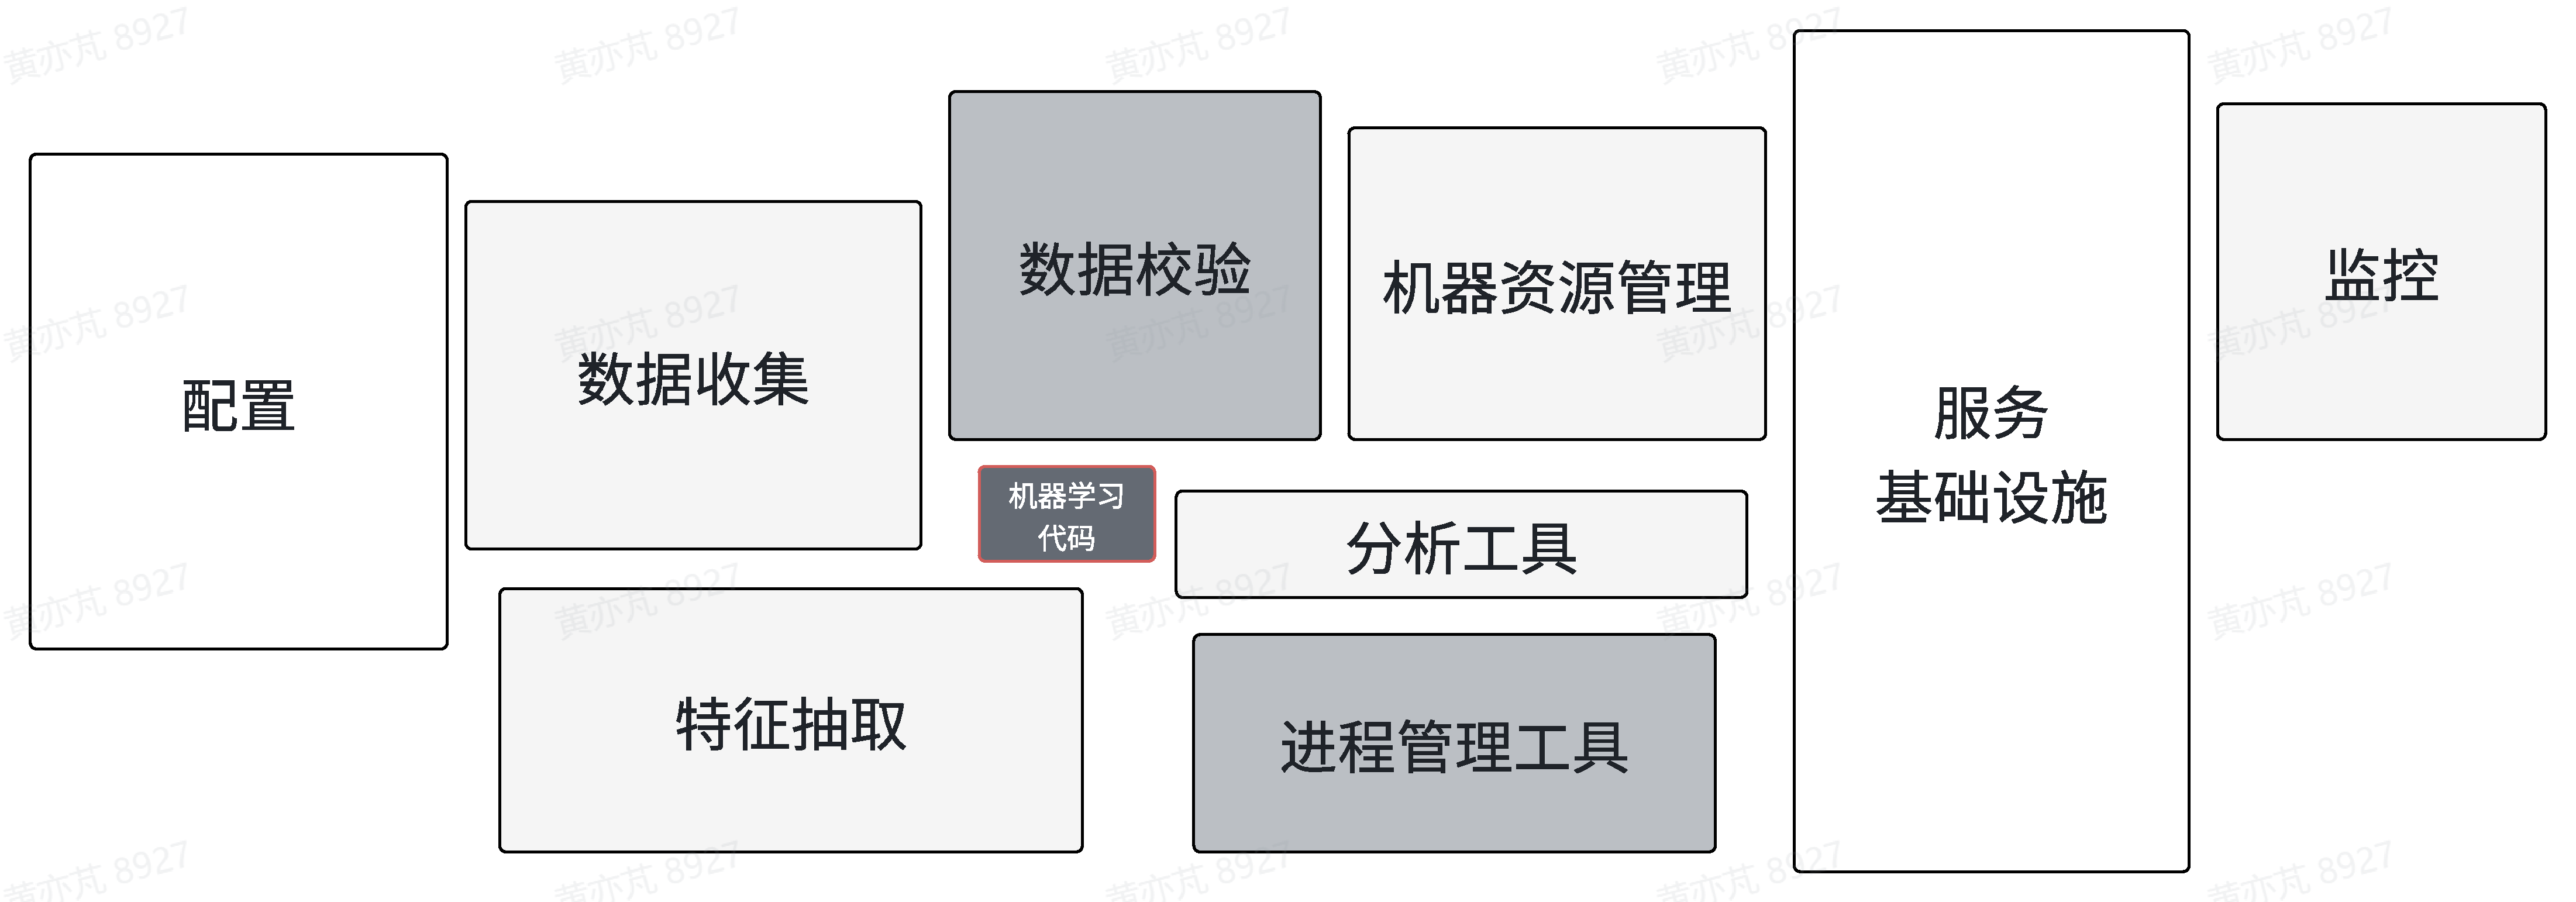
\includegraphics[width=0.98\linewidth]{ml-system-components.pdf}
  \caption{谷歌提出的机器学习系统组成}
  \label{fig:mlcomponents}
\end{figure}

人类的技术发展总是伴随着工程化的进程:从人力种植到机械耕作、从手工制造到工业生产、从编程开发到软件工程等等。
其中的关键是工具手段的出现和演进以及流程的标准化和自动化,以支撑技术的规模化应用。
其核心就是提高生产效率,从而解放生产力,降低生产成本,提高产品质量。
在机器学习领域,工程化的进程也是必然的,也是迫切的。
正如谷歌在机器学习系统设计的奠基性理论研究中所提出的,真实世界的机器学习系统中包含广阔而复杂的工程化基础设施,机器学习代码只是系统中很小的一部分,如图\ref{fig:mlcomponents}。
在模型核心技术研发的层面上,数据准备、算法开发、模型训练、模型评估等环节需要工具手段的辅助,以提高研发效率和模型性能;
在模型应用落地的层面上,模型部署、模型监控、流程自动化、业务应用集成等环节更需要工程化的系统软件支撑,以保证应用的稳定性、可靠性和可维护性。

【与软件工程的不同】
模型结构复杂、训练数据多、参数量大、随机性强

【为什么云原生】

需要注意的是,一些文献中将PyTorch、TensorFlow等机器学习计算框架称为机器学习平台,易与本文的研究对象混淆。
本文研究的机器学习平台是指支撑机器学习研发和应用的软件工具系统,依托于硬件基础设施(或称硬件平台,亦与本文中的平台不同),支持在平台中使用PyTorch、TensorFlow等机器学习计算框架进行模型训练、推理等计算作业。


%
\section{国内外研究现状}

TBD

\subsection{理论方法}

在实际的研发工作当中,模型开发过程难复现、实验程序难复用等问题频繁出现,导致大量的重复劳动,研发可持续性较差. Fursin等人\cite{Fur16}提出了一套模型研发产出的标准框架,规定了环境、算法、程序、流水线等相关内容的定义方式,研发人员可基于此形成研发项目数据库,支撑研发过程中产生的组件、工具、流程的复用,为团队协作提供基础,进而保障研发的可持续性. 


\subsection{工具系统}

针对机器学习应用落地的难题,一些研究工作体现在端到端的机器学习平台上\cite{Bay17, Sal18},机器学习模型的研发只是其中的一个环节。
平台的功能覆盖数据、模型训练和验证、应用部署和监控等方面,期望打通从数据接入到业务应用运维的机器学习完整工作流\cite{Ame19},满足机器学习应用快速上线并形成稳定服务的需求。
追求落地固然是机器学习技术的主要目标,但从根源上,如何使机器学习研发更高效是亟待突破的首要方向,将会对应用落地带来诸多裨益。

Kumar等人\cite{Kum16}将传统机器学习的模型开发过程抽象成特征工程、算法选择和参数调优等3项关键步骤,统称为“模型选择”(Model Selection),并基于此概念提出一种模型选择管理系统框架,包括声明式实验构建、运行时计算优化、模型来源管理与分析等功能,支撑高效的机器学习实验。
Tsay等人\cite{Tsa22}提出了人工智能实验数据库,着重针对研发过程可复现性问题,通过对实验元信息的建模、抽取和关联,聚焦实验产物及其生成过程的完整详细信息,保障从数据处理到模型实验的复现。
同样在研发过程方面,Sridhar等人\cite{Sri18}提出了模型治理的概念及相关系统,覆盖了机器学习模型开发与部署中的模型血统梳理、可复现性、审计、伸缩等需求,旨在帮助研发人员明确模型的产生路径及其在生产环境中的用途和效果,从而更好地复现研发方案、诊断实验过程中存在的问题。


模型是机器学习研发阶段最核心的产物,模型管理的重要性不言而喻. 模型管理系统在不同领域、不同应用场景下面临着诸多挑战\cite{Sch15, Scu15},近年来得到了学术界的广泛关注。
Vartak等人\cite{Var16}提出一种模型管理系统,以代码侵入的方式对实验进行跟踪,并对模型进行统一存储和索引,为用户提供共享、查询、分析等功能,帮助研发人员梳理模型研发过程、找寻规律并建立整体视角。
Schelter等人\cite{Sch17}则提出一种非侵入式模型跟踪方法,可针对一些机器学习框架自动进行实验记录,并提取出数据集、超参数、模型等机器学习常见资产的元信息,支撑实验的对比和复现以及模型血统分析。
Miao等人\cite{Mia17}针对深度学习模型研发提出了一套模型生命周期管理平台,更多地关注了模型快速迭代过程中的版本控制以及模型的社区式共享机制,并搭配了一种领域专用语言用以高效地检索和查询平台中的模型资产。
此外,该平台内置了一套模型来源管理模块,以图数据库的形式帮助用户记录、管理和梳理深度学习模型开发的过程。

产业界近些年也涌现了一批实验跟踪与模型管理的系统或平台\cite{wandb, neptuneai, huggingface},在模型资产管理和团队协作上的实践经验对模型研发管理系统的学术研究具有指导意义。

上述相关研究工作普遍在算法管理、计算环境管理、研发团队分工协作、实验方案的细粒度跟踪等方面存在不足之处:
(1)现有系统往往将机器学习算法视为传统软件代码,全权交由用户以通用的代码管理系统(例如GitHub)进行管理,缺乏对算法的资产化管理,进而无法有效地与模型、数据集等其他机器学习核心资产形成有机关联;
(2)同样地,现有系统也缺乏对计算环境的资产化管理,难以保证多次计算任务中环境的一致性;
(3)团队协作被广泛纳入现有系统的功能板块中,但往往仅限于团队成员间的资源共享机制,缺乏团队的组织架构管理以及任务的分工指派;
(4)类似地,实验跟踪虽然是现有系统的基本功能,但一般只能跟踪算法代码的提交信息,在探索式、迭代式的模型调试过程中,用户往往不会对每次细微的改动均做提交,现有系统便无法完整跟踪到每一次的方案变更。
本文提出的Anylearn机器学习研发管理系统在资产管理、团队协作、研发过程跟踪的功能框架下,研究并解决了相关工作存在的这些问题.

%
\section{研究内容与主要贡献}

TBD


%
\section{本文结构安排}

TBD
